\section{$\text{H}_2$/$\text{O}_2$ reaction kinetics: high-dimensional case}
\label{sec:app}

For the high-dimensional case, we aim to investigate the impact of the uncertain
pre-exponents ($A_i$'s) as well as the activation energies ($E_{a,i}$'s) on ignition 
delay during the H$_2$/O$_2$ reaction. The $A_i$'s were considered to be uniformly
distributed in the interval, $[0.9A_i^\ast, 1.1A_i^\ast]$. The $E_{a,i}$'s for all
reactions except $\mathcal{R}_6$ -- $\mathcal{R}_9$ and $\mathcal{R}_{13}$ (due to 
zero nominal values for $E_a$)
were considered to be uncertain and uniformly distributed in the interval: 
$[0.99E_{a,i}^\ast, 1.01E_{a,i}^\ast]$. The nominal values, $A_i^\ast$ and $E_{a,i}^\ast$
corresponding to the different reaction rates are provided in~\cite{Yetter:1991}. 

The gradient-based approach discussed earlier in~\ref{sub:grad} was used to compute the
active subspace. Using the iterative procedure, the convergence of the eigenvectors
was examined by tracking $\max(\delta \hat{\mat{W}}_{1,j}^{(i)})$, plotted in 
Figure~\ref{fig:conv_app} (right). In Figure~\ref{fig:conv_app} (left), individual
components of the converged eigenvector are illustrated. The convergence was established using
a $\tau$ value of 0.02. Finite difference was used to compute model gradients at 40 samples in
the input domain. Hence, a total of 1360 model evaluations were required for this purpose.  
%
\begin{figure}[htbp]
 \begin{center}
  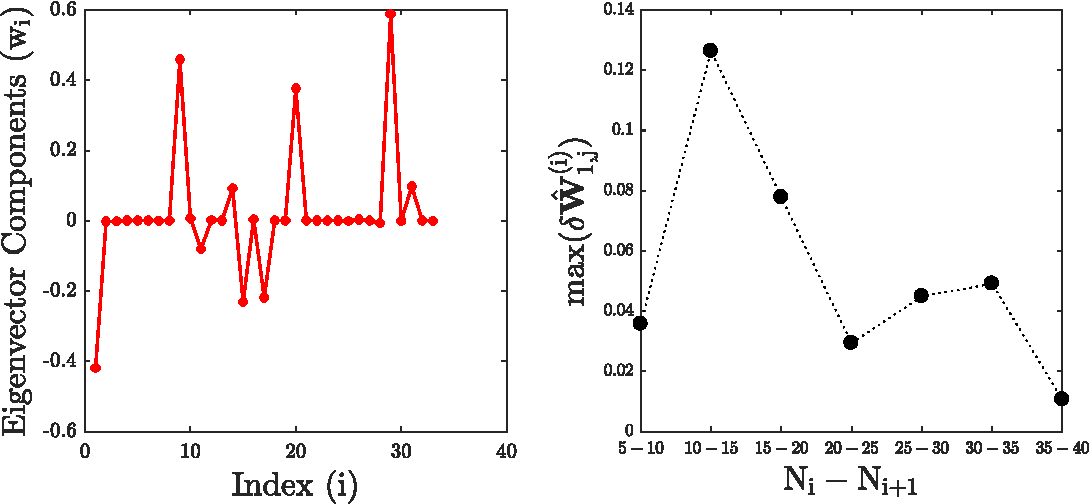
\includegraphics[width=0.8\textwidth]{./Figures/eigv10}
\caption{Left: An illustrative comparison of individual components of the converged dominant eigenvector obtained
using the two approaches discussed in~\ref{sub:grad} and~\ref{sub:gradfree}. Right: The quantity,  
$\max(\delta \hat{\mat{W}}_{1,j}^{(i)})$
is plotted for successive iterations to illustrate the convergence behavior.}
\label{fig:conv_app}
\end{center}
\end{figure}
%
 
In Figure~\ref{fig:hd} (left), we illustrate the resulting eigenvalue spectrum. The second eigenvalue is
found to be roughly two orders of magnitude smaller than the first, indicating that the active subspace
is 1-dimensional. This is further confirmed by the SSP plots in Figure~\ref{fig:hd} (right). Specifically
in the case of gradient-based approach, the SSP exhibits a linear variation that is reasonably
captured by its linear fit, $\tilde{G}$. Whereas, the SSP based on the gradient-free approach
is relatively more scattered. Consequently, the linear fit exhibits a discrepancy with the corresponding
fit for the gradient-based SSP. 
%
\begin{figure}[htbp]
 \begin{center}
   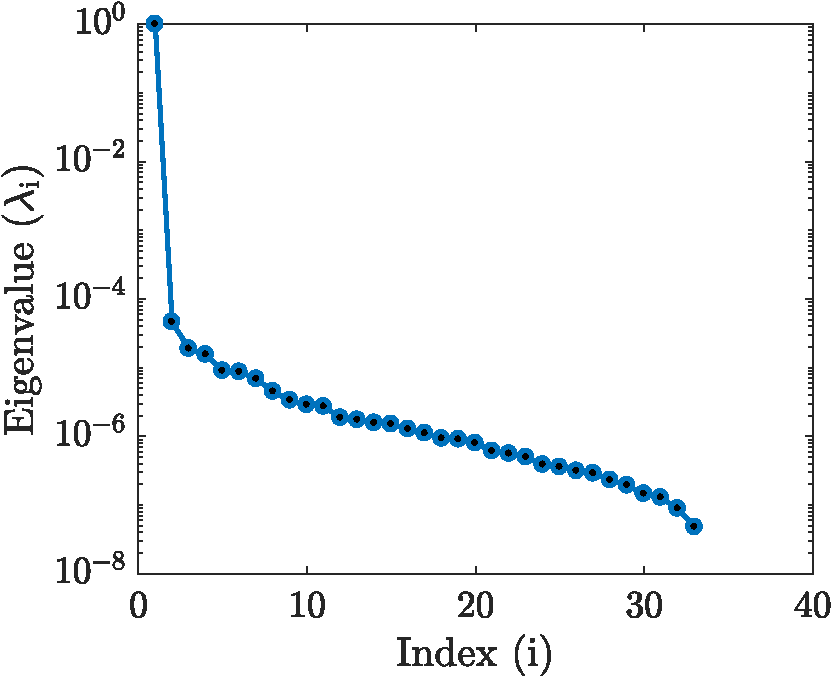
\includegraphics[width=0.45\textwidth]{./Figures/eig_33D}
   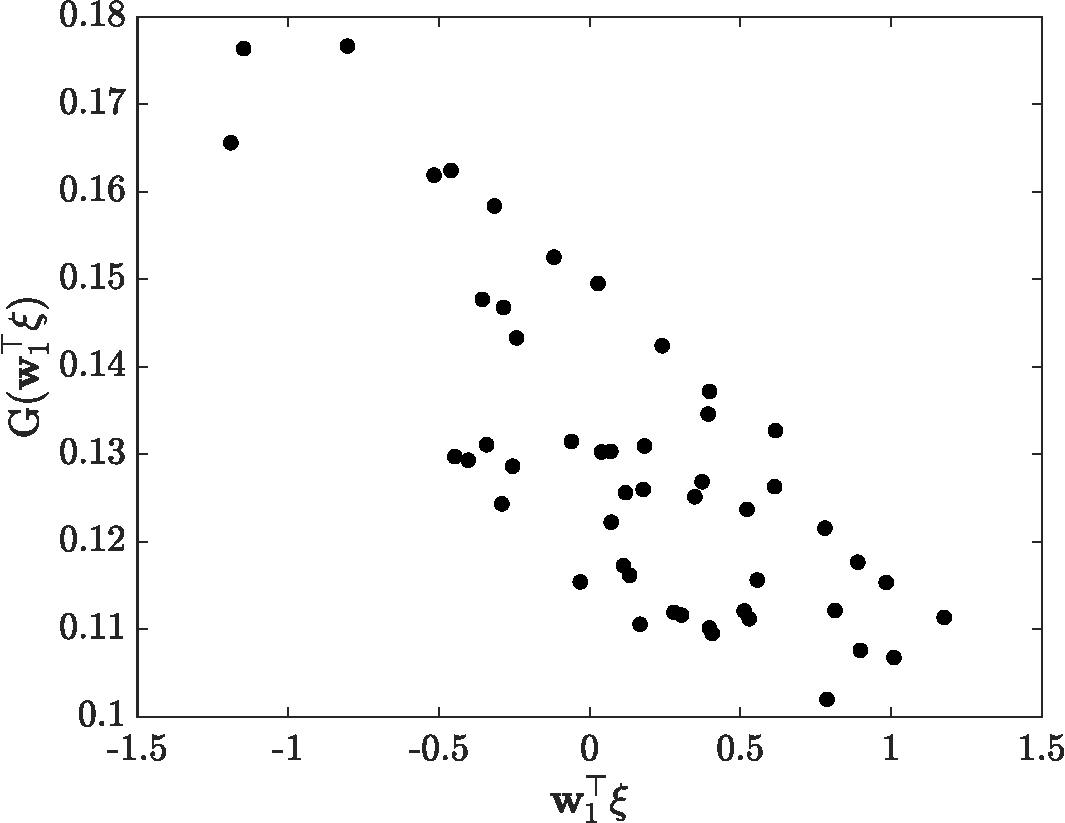
\includegraphics[width=0.45\textwidth]{./Figures/ssp_33D}
\caption{Left: Eigenvalue spectrum of $\hat{\mat{C}}$. Right: SSP of the computed active subspace, and the
corresponding 1-D linear fit.} 
\label{fig:hd}
\end{center}
\end{figure}
%
We plot the normalized activity scores as well as the total Sobol' indices for the 33 uncertain 
rate-controlling parameters in Figure~\ref{fig:as_33D}. Note that the normalized activity scores
as well as the Sobol' indices
were evaluated using respective 1-dimensional surrogates for the two approaches.
%
\begin{figure}[htbp]
 \begin{center}
  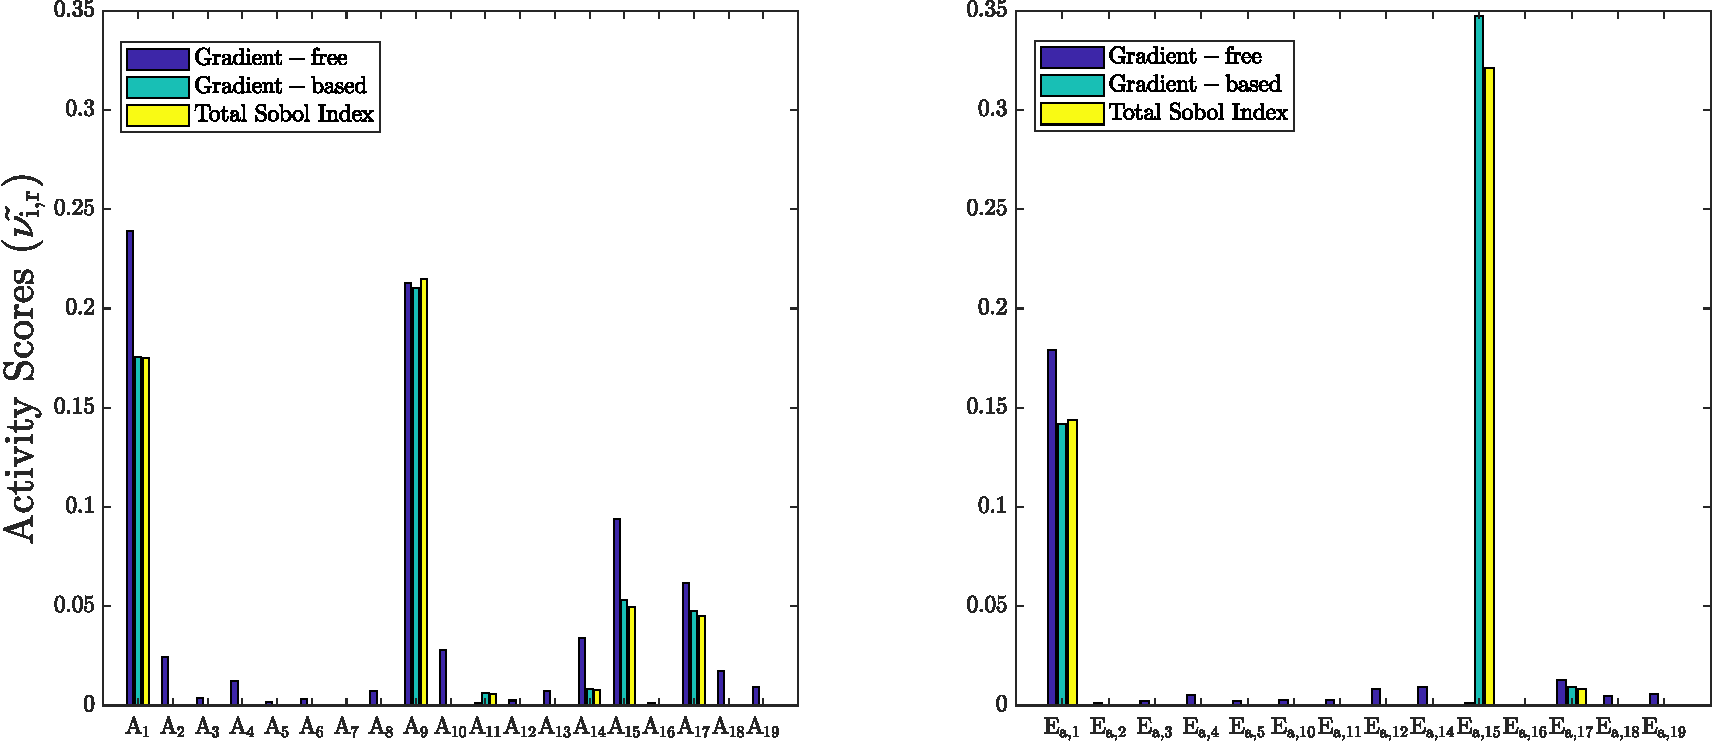
\includegraphics[width=0.8\textwidth]{./Figures/as_33D_new}
\caption{A bar-graph illustrating individual activity scores for the uncertain $A_i$' (left) and $E_{a,i}$'s (right).}
\label{fig:as_33D}
\end{center}
\end{figure}
%

Several useful inferences can be drawn from the above plot. Firstly, the total Sobol indices are found to be
consistent
with the normalized activity scores evaluated using the gradient-based approach. Whereas, the gradient-free
approach yields consistent results for the $A_i$'s, it does not capture the sensitivity associated with
$E_{a,15}$. While this observation bolsters our confidence in the gradient-based approach, it clearly
underscores the shortcoming of the gradient-free approach. Numerical errors are incurred when approximating
the model gradients using the local linear approximation in this case. In~\ref{sub:verify}, we further assess the
suitability of the gradient-free approach in quantifying the uncertainty in the ignition delay. 
Secondly, our findings indicate that   
the ignition delay is predominantly sensitive towards $A_1$, $A_9$, $E_{a,1}$, and $E_{a,15}$ and 
moderately sensitive towards $A_{15}$ and $A_{17}$. Sensitivity towards the remaining uncertain inputs is
found to be low or negligible. Note that this observation can also be exploited for reducing the 
dimensionality of the problem from 33 inputs to 4-6 inputs depending upon the required level of accuracy.
The sensitivity-driven dimension reduction for uncertainty quantification has been
discussed in our earlier effort~\cite{Vohra:2018}. In this work, however, we focus on dimension reduction using the active 
subspace approach which is shown to yield even greater scope for dimension reduction i.e. from 33 to 1. Furthermore, we have
shown that the dominant eigenspace can be used to approximate global sensitivity measures with no additional effort.
The accuracy of the 1-dimensional surrogate, $\tilde{G}$, obtained using the two approaches is assessed in the following section. 

\subsection{Surrogate Verification}
\label{sub:verify}

The 1-dimensional surrogate ($\tilde{G}$) is investigated for its accuracy as well as the ability to capture the 
uncertainty in the
model output in two ways. Firstly, we estimate the relative L-2 norm of the discrepancy~($\varepsilon_d$)
between estimates of ignition delay in the case of H$_2$/O$_2$ reaction, obtained using the 
model output and the surrogate in the following equation:
%
\be
\varepsilon_d = \frac{\|G(\bm{\xi}) - \tilde{G}(\bm{\xi})\|_2}{\|G(\bm{\xi})\|_2}
\ee
%
The relative norm, $\varepsilon_d$ was estimated to be 1.35$\times10^{-2}$ and 1.02$\times10^{-1}$
using $\tilde{G}$ from the gradient-based approach and the gradient-free approach respectively. Hence,
an order of magnitude increase in $\varepsilon_d$ was estimated in the case of gradient-free approach.
Model evaluations ($G$) at 10$^{4}$ samples in the input domain were used for this purpose. 
Hence, in the norm-sense, it can be said that the 1-dimensional surrogate in the active subspace, obtained
using the gradient-based approach is remarkably accurate with a relative error of less than 1.5$\%$.

Secondly, we verify the accuracy of the two surrogates in a probabilistic setting. In particular, we compare 
probability density functions (PDFs) obtained using the true set of model evaluations, and 1-dimensional
surrogates from the two approaches, in Figure~\ref{fig:pdf_33D}. Note that the three PDFs were evaluated 
using the same set of 10$^4$ samples in the cross-validation set. 
%
\begin{figure}[htbp]
\begin{center}
\begin{minipage}[htbp]{.25\linewidth}
\vspace{0pt}
%\centering
\hspace{-25mm}
\begin{tabular}{ccc}
\toprule
$\textbf{Distribution}$ & $\mu$ & $\sigma$ \\ 
\bottomrule
$G$~(Model) & 0.133 & 0.0198 \\
$\tilde{G}$~(Gradient-based) & 0.133 & 0.0196 \\
$\tilde{G}$~(Gradient-free) & 0.133 & 0.0167 \\
\bottomrule
\end{tabular}
\end{minipage}
\hspace{5mm}
\begin{minipage}[htbp]{.25\linewidth}
\vspace{0pt}
%\centering
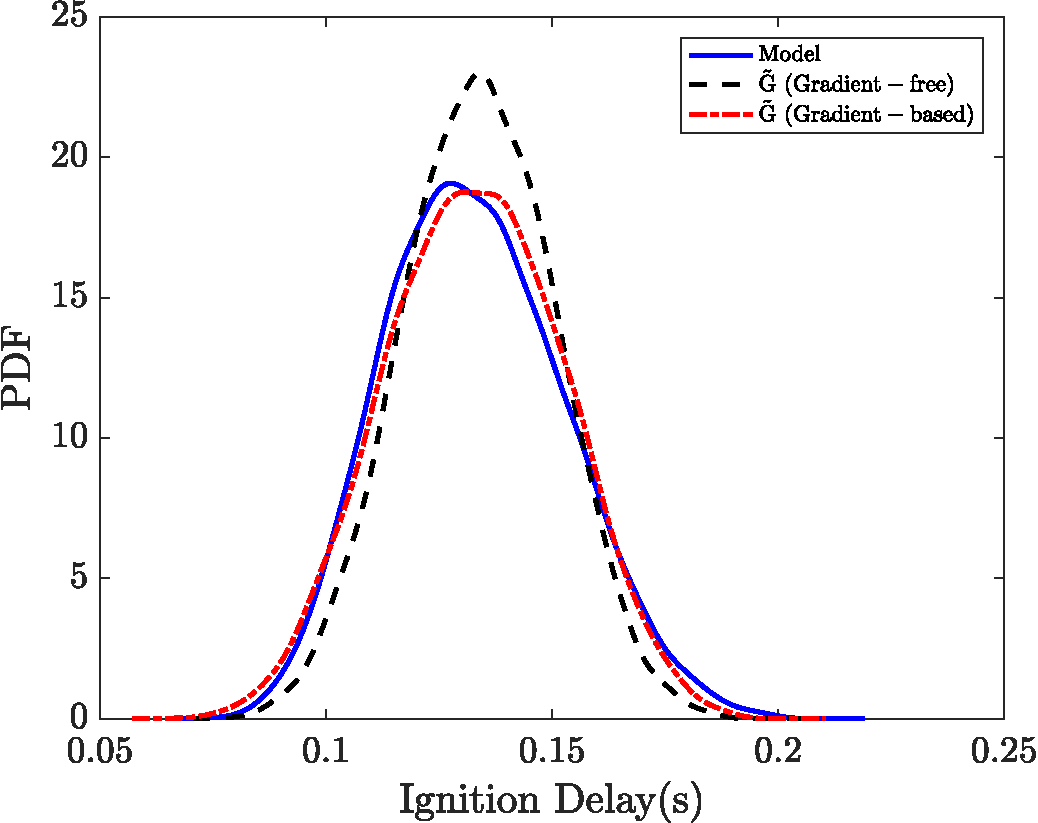
\includegraphics[width=3.0in]{./Figures/pdf_comp_id_1e4}
\end{minipage}%
\end{center} 
\caption{Left: Table providing the mean ($\mu$) and the standard deviation ($\sigma$) corresponding to
the three PDFs using evaluations
at 10$^4$ samples in the cross-validation set. Right: A comparison of the PDFs of ignition delay, obtained using model 
evaluations (solid line) and 1-dimensional surrogates using the gradient-free approach (dashed line) and the gradient-based
approach (dashed-dotted line). The same set of 10$^4$ samples in the cross-validation set were used in each case.}
\label{fig:pdf_33D}
\end{figure}
%
%
%\begin{figure}[htbp]
% \begin{center}
%  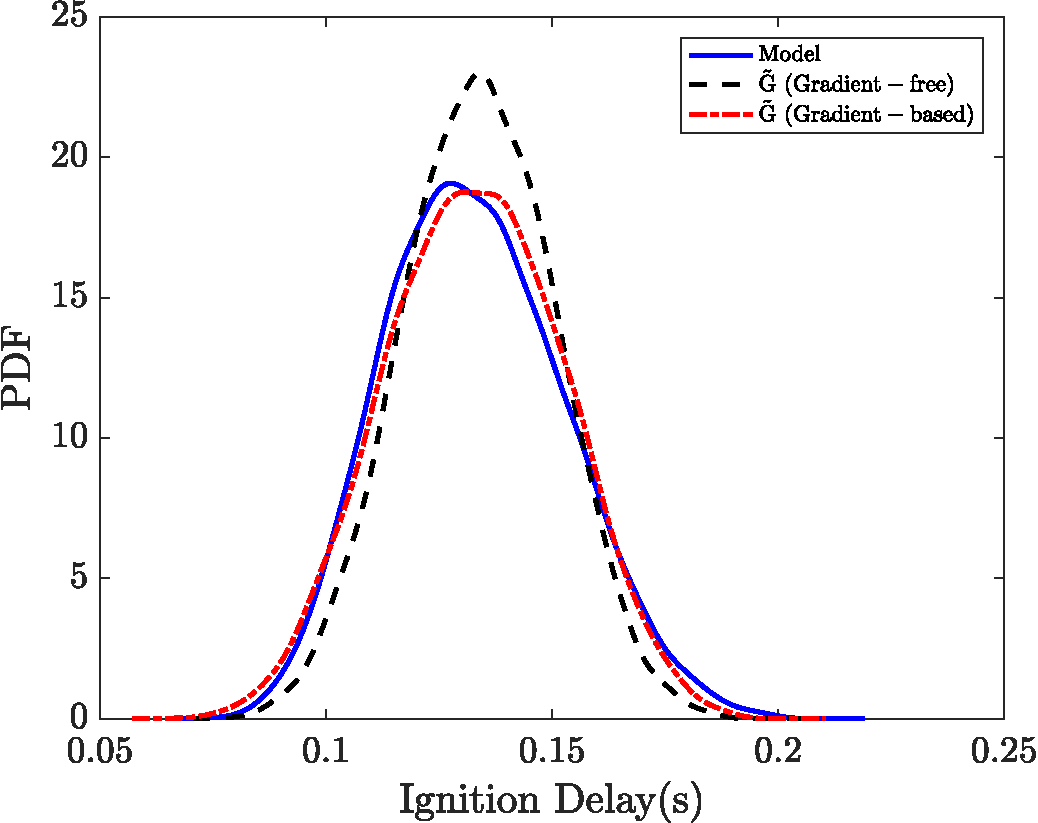
\includegraphics[width=0.45\textwidth]{./Figures/pdf_comp_id_1e4}
%\caption{A comparison of the PDFs of ignition delay, obtained using model evaluations (solid line) and
%1-dimensional surrogates using the gradient-free approach (dashed line) and the gradient-based approach
%(dashed-dotted line). The same set of 10$^4$ samples in the cross-validation set were used in each case.}
%\label{fig:pdf_33D}
%\end{center}
%\end{figure}
%
The PDFs based on the model evaluations and the gradient-based approach are nearly identical, confirming
the existence of a 1-dimensional active subspace as well as the accuracy of the gradient-based approach. 
Whereas, the PDF based on the gradient-free approach is observed to show consistency with the true PDF in the modal
estimate; it underestimates the spread in the ignition delay. Specific values of the mean and the standard deviation
in each case are provided in the table in Figure~\ref{fig:pdf_33D}. Hence, the three PDFs are found to be
consistent in their prediction of mean value of the ignition delay.  The standard deviation estimates based on model
evaluations and the gradient-based approach are found to be in close agreement, whereas, it  is accurately estimated
by the gradient-free approach only upto the first significant figure. 

%\subsection{Surrogate-induced risk analysis}






























